\section{Overview}

When trying to solve a problem using Classification, there are two significant algorithmic approaches that are considered, each with beneficiaries and adversaries that may also go hand-in-hand. 

For instance, the approach of using a decision tree-based model for identifying malicious code seems appealing – resembling a flowchart. 
As Figure 4 below shows, a file can be inputted into the algorithm, where it is analysed for certain attributes that have been pre-determined as malignant or not. 

 \begin{figure}[ht]
  	\centering
 	\label{fig1:example-flowchart-dt-ml}
 	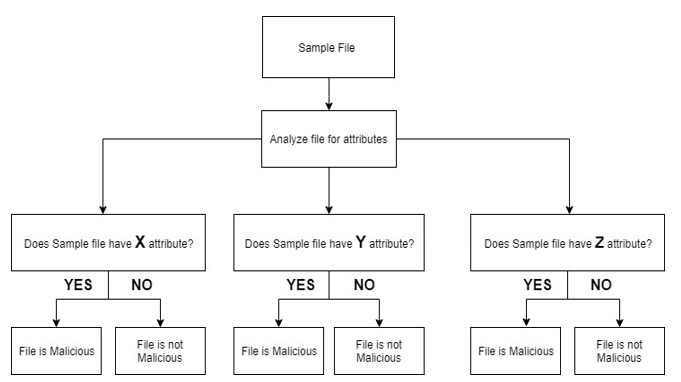
\includegraphics[width=\textwidth]{/Methodology/flowchart-decision-tree}
 	\caption{An example Flowchart illustrating decision-tree based Machine Learning.}
 	
 \end{figure}